\documentclass{article}
\usepackage{polyglossia}
\setmainlanguage{english}
\setotherlanguage{tamil}
\setdefaultlanguage{english}
\usepackage{graphicx}
\usepackage{array}
\usepackage{tabularx}
\graphicspath{ {images/} }
\usepackage{fontspec}
\newfontfamily\tamilfont[Script=Tamil,ExternalLocation]{TAMu_Kadampari.ttf}
\newcolumntype{Y}{|>{\centering\arraybackslash}X}
\title{TAMIL TEXT TO ENGLISH EMOTIONAL SPEECH CONVERSION WITH UNL FOR TRANSLATION
}


\author{B.ARCHANA - 2011103505 \\ M.R.SIVA - 2011103536\\R.JAYAVASANTH-2011103562\\ \\ \\ \\ \\ \\ \\ \\ \\ \\ \\ \\ \\ \\ \\ \\ \\ \\ \\ \\ \\ \\ \\ \\ \\ \\ \\ \\ \\ \\ \\ \\ \\ \\ \\ \\
Project Guide : Dr. Rajeswari Sridhar\\Asst. Professor (Sr. Grade)\\Department of Computer Science and Engineering,\\
Anna University, Chennai - 25}
\usepackage{geometry} 
\geometry{ 
a4paper, 
total={210mm,297mm}, 
left=30mm, 
right=30mm, 
top=30mm, 
bottom=20mm, 
}

\begin{document}
\maketitle
\newpage
\tableofcontents

\newpage
\section{Introduction}\large
This project in the field of Natural Language Processing aims at
translating an input Tamil sentence into an equivalent spoken English
translation of the sentence. This brings together two major domains in
NLP,i.e, machine translation and TTS(Text to Speech). Natural
Language Processing is the field of computer science that deals with
interactions between computer and human languages. One of the aim
of NLP is ”Natural Language Understanding”, i.e., to enable computers
to derive meaning from human language input. Computational
linguistics is a sub domain under NLP, which focuses specifically on
language related work such as language modelling, representation.
Machine Translation is one such field of computational linguistics.
Machine Translation involves the development of software for
translation of given text from a source language to the target
language.
\section{Problem Statement}\large
Given a Tamil sentence as input, the project will translate it into its corresponding English sentence with no loss in meaning while preserving the semantic structure of English.The translated sentence would be voiced over with a humanised robotic voice. Given a batch of sentences ( document input ), each sentence would be processed and translated and synthesised into speech with emotion.
\section{Project Description}\large
The first phase of the project i.e,conversion of Tamil input text
into English is done by converting Tamil text into the Universal
Networking Language representation and then converting from UNL into
the equivalent English form. Here UNL is used as the pivot language in
between the Tamil and English languages. Since, UNL is
language-independent, it offers a very flexible platform for the
representation of knowledge and thus gives great scope for research,
in conjunction with the rich language of Tamil, that we have
undertaken in our project.
The second phase of our project takes the converted English text and
processes it with a Text-To-Speech Engine, to convert it into speech.
This TTS system is modified at signal level so as to incorporate
emotion, to make the robotic speech more humanised. The given text
is transformed into speech with the necessary prosody,stress and
intonation marked so as to add emotion to the text.
\section{Literature Survey}\large
\begin{enumerate}
\item \textbf{Dhanalakshmi V., Anand kumar M., Soman K. P. and Rajendran S., \textit{"Postagger and Chunker for Tamil Language"}, Proceedings of the 8th Tamil Internet Conference, Cologne, Germany, 2009.}
\\This paper makes use of machine learning techniques to carry out POS tagging of tamil sentences. A custom tagset was developed to annotate the Tamil corpus for training and testing. Customised tagset reduces time and complexity increasing tagging accuracy. We follow a customized tagset as discussed in this paper to reduce complexity.

\item \textbf{Rajeswari Sridhar, Sugadev C, Mani Murugesan P, Vignesh N T,  \textit{"A hybrid approach to Tamil Morphological generation"}, 13th International Tamil Internet Conference, pp 101- 105, Pondicherry, 2014.}
\\This paper describes a rule based approach for morphological generation using a Suffix table. In root word analysis the suffix table discussed in this paper becomes the Inflection table and upon removing those inflections root words can be obtained.

\item \textbf{T.Dhanabalan, K.Saravanan, T.V.Geetha, \textit{“Tamil to UNL EnConverter”},Proc. Int. Conf. on Universal Knowledge and Language, 1-16,2002}
\\This paper defines all the possible relations that can exist between two UNL nodes based on the suffixes of words but it doesnot give much detail about the attributes of a UW. It handles the construction of Simple Nodes only.We would be using the rules given in this paper to construct the relations between two UWs.

\item \textbf{J Balaji, T V Geetha, RanjaniParthasarathi,  MadhanKarky, \textit{“Morpho-Semantic Features for Rule-based Tamil Enconversion”},International Journal of Computer Applications 26 (6), 11-18,2011} 
\\TThis paper elaborates on the rules for forming UNL graphs from suffixes. However this paper does not consider the relations associated with complex and compound tamil Sentences.It doesnot handle the cases where suffixes are implicit or hidden.We would adopt few rules from this paper on creating the Simple Nodes.


\item \textbf{Balaji J, Geetha T V, RanjaniParthasarathi, \textit{“Semantic Parsing of Tamil Sentences”},Workshop on Machine Translation and Parsing in Indian Languages (MTPIL), 24th International Conference on Computational Linguistics COLING 2012}
\\This paper talks about identifying the subgraphs in a sentence using certain inflections that corresponds to plt,mod relations.But it doesnot enunciate the cases, where punctuations could be helpful in identifying the sun-graphs that could be formed.

\item  \textbf{Tristan Bowles,SandraPauletto,  \textit{“Emotions in the Voice Humanising a Robotic Voice”}, In Proceedings of the 7th Sound and Music Computing Conference, Barcelona, Spain, 2010.}
\\This paper deals with how parameters such as fundamental frequency, amplitude are affected by speech with emotions such as anger, sadness and happiness.These parameters are studied in this project using Matlab and Praat in order to understand the exact variations that take place in the case of emotional speech, and how it differs among different emotions. In this project, emotions are analysed at the word level instead of the sentence level approach that was followed in this paper.


\item \textbf{Sudhakar Sangeetha, Sekar Jothilakshmi,  \textit{“Syllable based  text to speech synthesis system using auto associative neural network prosody prediction”}, In International Journal of Speech Technology, Vol-17, Issue-2, pp 91-98, 2014.}
\\This paper describes a successful attempt to detect prosody from text using five layer auto associative neural network. The prosodic features extracted from the text will be used for the prosody generation in speech.A neural network can thus be constructed to model the variations in parameters of emotional speech. 
\end{enumerate}

\section{Specifications} \large
PLATFORM - Windows 64 bit operating system\\
\\Tools used
\begin{itemize}
\item Matlab R2011a
\item Audacity
\item PRAAT
\item Simple NLG
\item Eclipse LUNA
\item ROUGE
\end{itemize}

\section{Top Level Block Diagram}\large
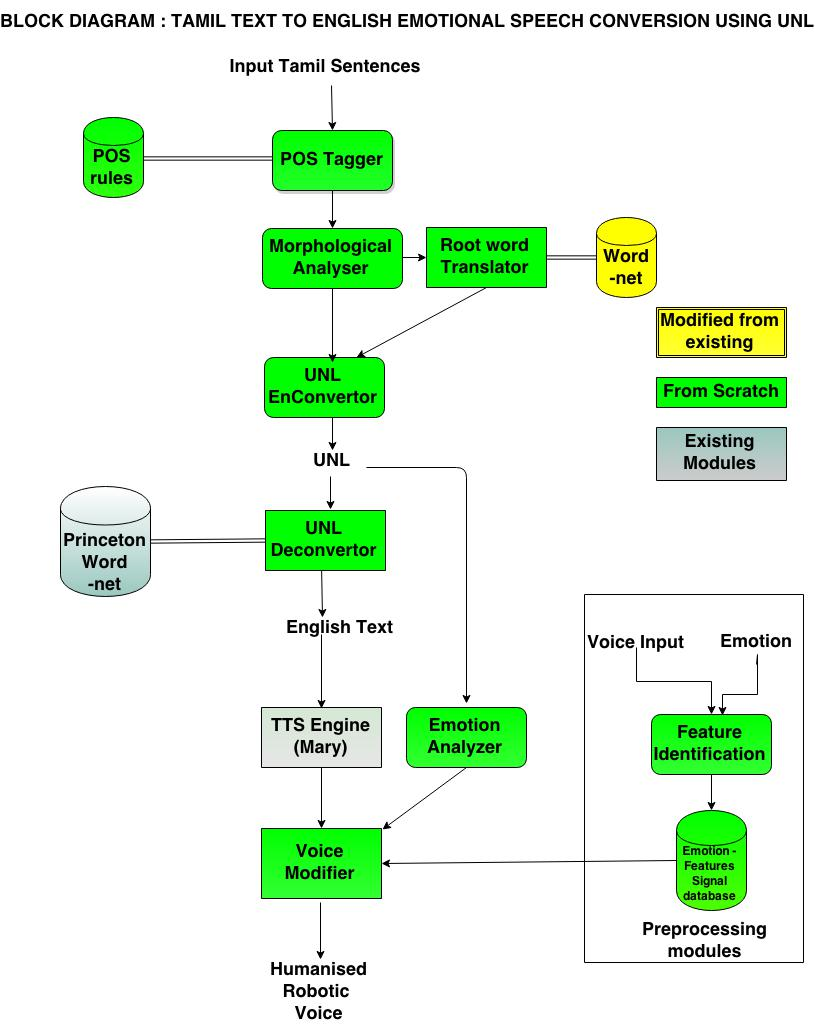
\includegraphics[width=\textwidth]{block}

\newpage
\section{Details Of Each Module} \large
%\begin{enumerate}
\subsection{POS TAGGING OF TAMIL SENTENCES}
The input sentence is given to this rule-based POS tagger which returns the part of speech of every word in the sentence.In Tamil there are ‘vallinammigumidam’ where a vallinamei \texttamil{(க், ச், த், ப்) } will be added to the inflected word, they are scanned from right to left. Once those vallinamei(if any) is removed, the inflections are used to determine the POS tags. A customised tagset tailored to fit the UNL relations and Enconversion module is created and used by this tagger. These tags are used in Morphological analysis and root word extraction.

\subsection{MORPHOLOGICAL ANALYSER}
Tamil is a morphologically rich language. A number of words can be formed from a root word by inflections. But only the root word will be mapped for translation and features like tense, gender and plurality can be extracted from the inflections which will be used in Deconversion to target language. A rule based morphological analyser has been developed for this purpose which takes inflected word with POS tag as input and it returns the root word which is the ‘Universal Word’ (UW) in the UNL representation.

\subsection{TAMIL WORDNET}
The wordnet consists of words and relationships between them such as hypernymy , hyponymy , holonymy , synonyms and antonyms etc., For the purpose of Word sense disambiguation - the wordnet becomes essential.For this purpose we would use the AU-KBC (Madras Institute of Technology) Tamil Wordnet along with few online dictionaries to fill in the English gloss attribute of the MIT wordnet. The wordnet would be deromanized before using. Also the wordnet will be converted to a Graph database format with Neo4j.

\subsection{UNL ENCONVERTER}
The process of converting Source text to UNL Graph is called Enconversion.UNL Graph are composed of nodes called as Universal Words (UW) and relations between them.Also each UW has one or more attributes attached to them.The output from a morphological analyser is processed using a manually defined set of rules to form UNL expressions.The root word of each important word in a sentence forms an UW and the suffixes attached to these words determine the relations between Uws. Some words including articles,prepositions and adjectives form attributes of these UWs.
\\Also the UWs that have to be processed together form a hyper node or a sub graph .The hypernodes are identified using suffixes of the Tamil words and a scope identifier is attached to these nodes for specifying them as a Hyper Node.

\subsection{UNL DECONVERTER}
The process of converting UNL Graph to target language text is called Deconversion. Deconversion is done with the help of a Natural Language Generator called Simple NLG.The UNL graph is anlaysed in hyper-node wise hierarchy and every time the Subject , Verb , Object , Adjective , Tense conveyed by the UNL is identified using the UNL relations and attributes.These are then fed to a SimpleNLG instance to generate the sentence.

\subsection{EMOTION-FEATURES DATABASE CONSTRUCTION}
This database consists of all features that have been extracted from the voice samples. The voice samples are obtained from 3 female speakers who have similar speech characteristics as that of Marytts' voice.  Since the output of the "MaryTTS" (Text to speech system) which has a female voice is to be modified, the voice samples are taken from female speakers. 7 sentences are recorded in a variety of emotions such as angry, happy, sad and neutral.  The voices are recorded in a fairly quiet room so as to avoid any external noise getting recorded. Then the sentences are read into Audacity, an audio analysis software in order to distinguish between the word boundaries clearly and to split them into audio files corresponding to each word. If excess noise has been recorded, then using the noise removal feature of Audacity, the audio sample can be made relatively noise free.\\
\subsubsection{FUNDAMENTAL FREQUENCY ESTIMATION}
Once the word samples are obtained, they are given as input to the MATLAB program in order to measure the dominant fundamental frequency F0 present in each word. They are recorded systematically in the features database. In order to make sure that the correct F0 values have been measured, it is carried out using 2 different approaches. 
\begin{itemize}
\item In frequency domain using cepstral analysis
\\The cepstrum is a Fourier analysis of the logarithmic amplitude spectrum of the signal.  If the log amplitude spectrum contains many regularly spaced harmonics, then the Fourier analysis of the spectrum will contain  a peak corresponding to the spacing between the harmonics: i.e. the fundamental frequency.
\item In time domain using autocorrelation 
\\The autocorrelation function for a section of signal shows how well the waveform shape correlates with itself at a range of different delays, thereby determining the periodicity in the waveform itself.
\end{itemize}
Once the F0 value has been determined, it can be used for pitch modification in the output of the text to speech synthesis system for prosody addition.\\
\subsubsection{DURATION OF EACH WORD }
This is measured using Audacity that has a millisecond calibration so that the exact duration of every word can be estimated.\\
\subsubsection{INTENSITY ESTIMATION}
Generally, words said with different emotions differ in the intensity with which they are spoken. For eg, when a person speaks with anger, there is a greater intensity in the voice than when compared to a person who speaks with sadness. So, this measurement is done with the help of PRAAT tool, that can accurately measure with what intensity the word was spoken. It is measured in decibels. 

\subsection{EMOTION IDENTIFICATION }
The emotion present in the sentence is calculated by using the output of the UNL which is annotated with the tone of the sentence. Various degrees of emotion can be identified based on the strength of the words that are used in the sentence. After this has been estimated, it is mapped onto one of the emotions that have been handled in the emotion-features database.

\subsection{VOICE MODIFICATION AND OUTPUT}
The output of the test to speech system is modified to add the emotion and prosody. The emotion features database is consulted and the corresponding values of various parameters (like fundamental frequency, intensity, duration etc) are calculated. Then the robotic voice is modified based on the values of these parameters to produce the humanised voice. 



\section{Description of Input and Output}\large
\begin{center}
\begin{tabularx}{\linewidth}{|@{}lYYYYY@{}|}
\hline\hline
MODULES & INPUT & OUTPUT\\
\hline
POS Tagger & \texttamil{அவன் புத்தகத்தை படிக்கிறான்} &  
\begin{itemize}
\item \texttamil{அவன்}– Subject, Pronoun
\item \texttamil{ புத்தகத்தை }- Noun
\item \texttamil{ படிக்கிறான் }- Verb
\end{itemize}\\
\hline
\item Morphological analyser &
\begin{itemize}
\item \texttamil{புத்தகத்தை} 
\item \texttamil{ படிக்கிறான் }
\end{itemize} &
\begin{itemize}
\item \texttamil{ புத்தகம்  }- Root
\item \texttamil{ ஐ  }- Noun Suffix
\item \texttamil{ படி }- Root
\item \texttamil{ கிறு  }- Present tense
\item \texttamil{ ஆன்  }-  Singular Male
\end{itemize}\\
\hline
Emotion-features signal database &
Sample audio file in .wav format having words in anger, happiness, sadness &
Values of fundamental frequency, intensity, word duration\\
\hline
EnConverter &
\texttamil{அவன் மருத்துவமனைக்குச் சென்றான்}
&
[UNL]
[W]
Kannan (icl>person) @masculine
Hospital (icl>place)
Go @past @entry
[/W]
2 agt 0
2 plt 1
[UNL]\\ 
\hline
DeConverter &
[UNL]
[W]
Kannan (icl>person) @masculine
Hospital (icl>place) 
Go @past @entry
[W]
2 agt 0
2 plt 1
[UNL] &
Kannan went to the hospital\\
\hline
Emotion identification &
UNL Relation graph &
Identified emotion\\
\hline
Voice modification and Output &
Output from TTS engine &
Prosody incorporated audio output\\
\hline
\end{tabularx}
\end{center}

\section{Algorithm}\large
\begin{enumerate}
\item POS TAGGER :
\begin{itemize}
\item Split the input sentence into words
\item Right to left scanning of words
\item Remove  “\texttamil{க்} || \texttamil{ச்} || \texttamil{த்} || \texttamil{ப்}” if any at the end
\item Assign tags based on the inflection at the end the result from wordnet
\end{itemize}
\item MORPHOLOGICAL ANALYSER :
\begin{itemize}
\item With the POS tag
\item Assign tense based on \texttamil{இடைநிலை}
\item Assign doer based on \texttamil{விகுதி}
\item Extract root word handle \texttamil{திரிதல், விகாரம் }
\end{itemize}
\item TRANSLATION :\\
E←element ( word , punctuation)\\
Seg←  Segmented Word\\
UW ← Universal Word\\
UNL ← Universal Networking Language\\
HN ← Hyper Node\\
Rel← UNL Relations\\
\begin{itemize}
\item Translate ( S [tamil] )\\
UNL = Enconvert( S [Tamil] )\\
S [English] = Deconvert( S [Tamil] )\\
\item Enconvert ( S [Tamil] ) \\
$For each e_{i} in S $\\
$Segroot , suffix [i] = MorphologicalAnalysis ( ei )$\\
$Seg[i] = SuffixPOSTagging ( Segroot , suffix [i] )\\ + PredictivePOSTagging (Segroot , suffix , suffix based POS [i] )\\
For each Si  in Seg[ i ]$\\
$UW [i] = root [Si]$\\
$attributes [i] = SuffixAnalysis ( Si )$\\
$For each UW[i],Seg[i] in UW,Seg$\\
$rel [k] = SuffixAnalysis ( S_{i} , S_{i + 1} ) + DomainAnalysis ( root [ S_{i} ] )$\\
$HN[j] = SuffixAnalysis( S_{i} , S_{i + 1} )$\\
$UNL = UW + Rel$\\
\item Deconvert ( S [Tamil] )\\
$For each  h{i} in Hypernode$\\
$For each r{i} in relations[]$\\
\hspace{200pt} $\hspace{200pt} \qquad Subject,verb,object,Adverb = RelationAnalysis( r{i})$\\
		$Sentence{i} = SimpleNLG(subject,verb,object,Adverb)$\\
         $Sentence = SimpleNLGClause ( Sentence{i to j} )$\\
\end{itemize}
\item EMOTION-FEATURES SIGNAL DATABASE CONSTRUCTION :\\
Estimation of fundamental frequency \\
-In frequency domain using cepstrum :
\begin{itemize}
\item (samples,sampling rate)] <-- wavread(audio file)
\item millisecond1 <-- sampling rate /1000
\item millisecond20<-- sampling rate /50
\item Y <-- Fast Fourier Transform( samples .* hamming (length (samples)))
\item Cepstrum<-- Fast Fourier Transform (log(absolute (samples)+eps))
\item (c, fundamental frequency) <-- max(absolute (Cepstrum (ms1:ms20))
\item Fundamental frequency <-- fs/(millisecond1+fx-1)
\end{itemize}
-In time domain using autocorrelation:
\begin{itemize}
\item (samples,sampling rate)] <--wavread(audio file)
\item millisecond2<-- sampling rate / 500 
\item millisecond20<-- sampling rate /50
\item rvalue<-- XCorrelation(samples, millisecond20)   
\item (rmaxvalue ,tx) <-- max(rvalue(millisecond2 : millisecond20))
\item Fundamental frequency <-- fs/(millisecond2+tx-1)
\end{itemize}

\item EMOTION IDENTIFICATION :
\begin{itemize}
\item EmotionLookup<- UNL graph output
\item Output <- Emotion
\end{itemize}

\item VOICE MODIFICATION :
\begin{itemize}
\item AccessEmotionFeaturesDatabase(Emotion)
\item Fundamental Frequency <- EmotionFeaturesDatabase
\item Intensity<- EmotionFeaturesDatabase
\item Duration<- EmotionFeaturesDatabase
\item ModifyVoice(Fundamental frequency, Intensity, Duration)
\end{itemize}
\end{enumerate}

\section{Evaluation Parameters for Modules}\large
\begin{center}
\begin{tabularx}{\linewidth}{|@{}lYYYYY@{}|}
\hline
MODULES & EVALUATION PARAMETERS \\ 
\hline\hline
	POS Tagger &  Comparison of efficiency between existing POS tagger - Kadhambam  and our output with Human judgement as reference.\\
\hline
Morphological Analyser &  Comparison of efficiency between existing analyser - Atcharam and our output with Human judgement as reference.\\
\hline
	Emotion-features signal database construction
& \begin{itemize}
\item The number of variations between the values of F0 determined in time domain and frequency domain.
\item The number of values of F0 that are harmonics i.e, multiples of fundamental frequency F0
\end{itemize}\\
\hline
	Voice Modification and Output & Using a public poll to determine
\begin{itemize}
\item  On a scale from 1 to 5 how emotional the final output is by comparing it with (robotic) output from Marytts.
\item What emotion is expressed by the output 
\item If the emotion conveyed by the input is the same as idetified from UNL.
%\item Number of times an emotion is correctly recognized. 
%\item Number of times an emotion is wrongly recognized.
\end{itemize}\\
\hline
\end {tabularx}
\end{center}
\textbf{Evaluation formulae} 
\begin{itemize}
\item POS Tagging\\
Percentage efficiency of\\ $POS\ Tagger =\frac {No\ of\ words\ correctly\ tagged\ by\ our\ tagger} {No\ of\ words\ correctly\ tagged\ by\ human\ reference}$\\
\item Morphological Analysis\\
Percentage efficiency of\\ $Morphological\ Analyser =\frac {No\ of\ root\ words\ correctly\ identified\ by\ our\ analyser} {No\ of\ root\ words\ correctly\ identified\ by\ human\ reference}$\\
\item \textbf{Word Error Rate}\\
It is a common metric for evaluation of the performance of the MT systems based on levenshtein distance.The output sentence is aligned using a dynamic string alignment algorithm and the word error rate is calculated as \\
$ WER = \frac { S + D + I }{ N } $ \\
or\\
$ WER = \frac { S + D + I }{ S + D + C } $ \\
where
\begin {itemize}
\item S is 	the number of substitutions, 
\item D is 	the number of deletions,
\item I is 	the number of insertions,
\item C is 	the number of the corrects,
\item N is 	the number of words in the reference $(N=S+D+C)$\\
\end {itemize}

\item \textbf{BLEU Score (Bilingual Evaluation Understudy )}\\
It is a n-gram co-occurence based MT evaluation system that verified how close the MT translated text is to , to a human translated reference.
N-gram precision in BLEU is computed as follows:\\

$p_{n} = \frac { \sum { C  \epsilon \textbraceleft Candidates \textbraceright }{} \sum{n-gram \epsilon C }{ Count _ {clip} (  n - gram )} }{ \sum{C  \epsilon \textbraceleft Candidates \textbraceright } \sum{n-gram \epsilon C }{} Count (  n - gram ) }$\\

Where $Count_{clip}(n-gram)$ is the maximum number of n-grams co-occurring in a candidate translation.\\ We would evaluate based on bigrams.

\item \textbf{ROUGE}\\
ROUGE, or Recall-Oriented Understudy for GistingEvaluation,is a set of metrics and a software package used for evaluating automatic summarization and MT systems.It was developed by Chin-Yew Lin while he was at the Information Sciences Institute of University of Southern California.Among various ROUGE methodologies , we will be using Rouge-L since it is different from any other methodology mentioned above.For a reference translation X of length m and the translated text Y of length N , the ROUGE - L score is computed as follows:
$R_{lcs} = \frac {LCS(X,Y)}{m}$\\
$P_{lcs} = \frac { LCS (X,Y) }{n} $\\
$F_{lcs}=\frac { ( 1 + \beta^2 ) R_{lcs} P_{lcs} } { R_{lcs} + \beta^2 P_{lcs} }$\\ 
Where LCS(X,Y) is the length of a longest common subsequence of X and Y, and $\beta=\frac{ Pl_{cs}}{Rl_{cs}}$ when $ \frac{\partial Fl_{cs}}{\partial Rl_{cs}}=\frac{\partial Fl_{cs}}{\partial Pl_{cs}}$
ROUGE - L can be determined easily with Rouge Software provided by Lin.\\

\item \textbf{METEOR (Metric for Evaluation of Translation with Explicit ORdering)}\\
It is based on the harmonic mean of unigram precision and recall , with recall weighted higher than precision. It also has several features that are not found in other metrics, such as stemming and synonymy matching, along with the standard exact word matching. The metric was designed to fix some of the problems found in the more popular BLEU metric, and also produce good correlation with human judgement at the sentence or segment level .It involves alignment of the reference text with the translated text.The the score is computed as 
$M = F_{mean} ( 1 - p ) $\\
where M denotes the scoreand p denotes the penalty computes as
$ p = 0.5 \frac {c} { u _ {m} ^3} $  \\
where c is number of chunks of data , $u_{m}$ is the number of unigrams that have been mapped.
\end{itemize}


\newpage
\section {Test cases}\large
\begin{itemize}
\item Test cases for Translation
\begin{enumerate}
\item Test case ID : TC-01\\
      \textit{Input}:\texttamil{ அவள்  பள்ளிக்குச் செல்கிறாள்.}\\
      \textit{Output:} She is going to school.\\

\item Test case ID : TC-02\\
      \textit{Input:}\texttamil{ கன்னகி  மதுரையை எரித்தாள்.}\\
      \textit{Output:} Kannagi burnt Madurai.\\
      
\item Test case ID : TC-03\\
      \textit{Input:} \texttamil{அவன் பந்து எரிந்தான்}.\\
      \textit{Output:} He threw a ball. \\
      
\item Test case ID : TC-04\\
      \textit{Input:} \texttamil{அவர்கள் அழகிய மானைக் கண்டனர்}.\\
      \textit{Output:} They saw a beautiful deer. \\

\item Test case ID : TC-05\\
      \textit{Input:} \texttamil{அவள் மகிழ்ச்சியில் ஒடினாள்.}\\
      \textit{Output:} She ran happily. \\

\item Test case ID : TC-06\\
      \textit{Input:} \texttamil{அவன் சோகத்தில் அழுதான்.}\\
      \textit{Output:} He wept in sorrow. \\

\item Test case ID : TC-07\\
      \textit{Input:} \texttamil{கண்ணன் கடையில் புத்தகம் வாங்கினான்..}\\
      \textit{Output:} Kannan bought a book in the shop. \\
    
\item Test case ID : TC-08\\
      \textit{Input:} \texttamil{வைகை மதுரையில் உதயமாகிறது.}\\
      \textit{Output:} Vaigai originates in Madurai. \\    
      
\item Test case ID : TC-09\\
      \textit{Input:} \texttamil{அவன் சென்னையைச் சேர்ந்தவன்.}\\
      \textit{Output:} He belongs to chennai. \\        
      
\item Test case ID : TC-10\\
      \textit{Input:} \texttamil{வேடன் கிளையின்கண் இருந்த பறவையைக் கொன்றான்.}\\
      \textit{Output:} Hunter killed the bird sitting on a branch.\\
            
\item Test case ID : TC-11\\
      \textit{Input:} \texttamil{நான் மருத்துவராக விரும்புகிறேன்.}\\
      \textit{Output:} I want to become a doctor. \\        
            
\item Test case ID : TC-12\\
      \textit{Input:} \texttamil{இன்று விடுமுறை.}\\
      \textit{Output:} Today is a holiday. \\             
            
\item Test case ID : TC-13\\
      \textit{Input:} \texttamil{சென்னை தமிழ்நாட்டின் தலைநகரம்.}\\
      \textit{Output:} Chennai is the capital of Tamil Nadu. \\        
            
\item Test case ID : TC-14\\
      \textit{Input:} \texttamil{அவன் வேற்றுகிரக விண்கலம் ஒன்றைக் கண்டதாகச் சொன்னான்.}\\
      \textit{Output:} He said that he saw an extra-terrestrial object.\\
            
\item Test case ID : TC-15\\
      \textit{Input:} \texttamil{இணையதளத்தில் இருந்து தமிழ்ப் பாடல்களைப் பதிவிறக்கம் செய்யாதே.}\\
      \textit{Output:} Do not download Tamil songs from the Internet. \\
\end{enumerate}
\item Test case for Voice modification\\
\textit{Input:} Speech without emotion, Identified emotion.\\
      \textit{Output:} Speech with 'identified emotion' incorporated. \\
\end{itemize}

\section {Screenshots}\large
Screenshots of Review 1 are attatched:
\begin{figure}[!ht]
\includegraphics[width=\textwidth]{image09.png}
\caption{Output of Morphological Analyser}
\label{fig:1}
\end{figure}

\begin{figure}[!ht]
\includegraphics[width=\textwidth]{enconverter.png}
\caption{Output of Enconverter and Deconverter}
\label{fig:2}
\end{figure}

\begin{figure}[!ht]
\includegraphics[width=\textwidth]{emotions.png}
\caption{Emotion parametric Analysis of a sentence}
\label{fig:3}
\end{figure}

\newpage
\section{References}\large
\begin{enumerate}
\item Sudhakar Sangeetha, Sekar Jothilakshmi,  \textit{“Syllable based  text to speech synthesis system using auto associative neural network prosody prediction”}, In International Journal of Speech Technology, Vol-17, Issue-2, pp 91-98, 2014.

\item Dave S., Parikh J. and Bhattacharyya P., \textit{"Interlingua Based English Hindi Machine Translation and Language Divergence, Machine Translation"}, Journal of Machine Translation, Volume 16, pp.251-304, 2001. 

\item Dhanalakshmi V., Anand kumar M., Soman K. P. and Rajendran S., \textit{"Postagger and Chunker for Tamil Language"}, Proceedings of the 8th Tamil Internet Conference, Cologne, Germany, 2009.

\item Rajeswari Sridhar, Sugadev C, Mani Murugesan P, Vignesh N T,  \textit{"A hybrid approach to Tamil Morphological generation"}, 13th International Tamil Internet Conference, pp 101- 105, Pondicherry, 2014.

\item T.Dhanabalan, K.Saravanan, T.V.Geetha, \textit{“Tamil to UNL EnConverter”},Proc. Int. Conf. on Universal Knowledge and Language, 1-16,2002.


\item J Balaji, T V Geetha, RanjaniParthasarathi,  MadhanKarky, \textit{“Morpho-Semantic Features for Rule-based Tamil Enconversion”},International Journal of Computer Applications 26 (6), 11-18,2011

\item Balaji J, Geetha T V, RanjaniParthasarathi, \textit{“Semantic Parsing of Tamil Sentences”},Workshop on Machine Translation and Parsing in Indian Languages (MTPIL), 24th International Conference on Computational Linguistics COLING 2012.


\item  Tristan Bowles,SandraPauletto,  \textit{“Emotions in the Voice Humanising a Robotic Voice”}, In Proceedings of the 7th Sound and Music Computing Conference, Barcelona, Spain, 2010.

\item Rajeswari Sridhar , Jayavasanth R,  \textit{"Tamil Wordnet based on hybrid approach"}, 13th International Tamil Internet Conference, pp 116- 121, Pondicherry, 2014.

\item Lin, Chin-Yew and Franz Josef Och. \textit{Automatic Evaluation of Machine Translation Quality Using Longest Common Subsequence and Skip-Bigram Statistics}, In Proceedings of the 42nd Annual Meeting of the Association for Computational Linguistics (ACL 2004), Barcelona, Spain, July 21 - 26, 2004.
\end{enumerate}


\end{document}
